\documentclass{article}

% 字体设置
\usepackage[no-math]{fontspec}
\setmainfont{Times New Roman}
\usepackage[UTF8]{ctex}
% \setCJKmainfont{Noto Serif SC}[ItalicFont=方正仿宋_GBK]
% \setCJKmathfont{Noto Serif SC}[ItalicFont=方正仿宋_GBK]

% 数学输入
\usepackage{amsmath}
\usepackage{amsfonts}
\usepackage{amssymb}
\usepackage{esint}
\usepackage{tikz}
\usepackage{latexsym}

% 排版设置
\usepackage{enumitem}
\usepackage{xcolor}
\usepackage{geometry}
\usepackage{float}
% \geometry{a5paper}
% \geometry{left=0.3cm, right=0.3cm, top=1.7cm, bottom=1.7cm}
\geometry{a4paper}
\geometry{left=1.9cm, right=1.9cm, top=1.7cm, bottom=1.7cm}

% 表格
\usepackage{array}
\usepackage{tabularx}
\usepackage{caption}
\providecommand{\tightlist}{\setlength{\itemsep}{0pt}\setlength{\parskip}{0pt}}
\usepackage{siunitx}

% 超链接
\usepackage{hyperref}
\urlstyle{rm}
\hypersetup{
    colorlinks=true, 
    linkcolor=black, 
    citecolor=black, 
    urlcolor=black, 
    bookmarks=true, 
    bookmarksopen=true, 
    bookmarksnumbered=true, 
}

% 标题和作者设置
\title{实验 4 \quad FIFO实验}
\author{Chen-Yuanmeng\thanks{Email: \url{chenyumeng23@mails.ucas.ac.cn}}}
\date{2024/12/5}

% 定义代码环境
\usepackage{listings}

\definecolor{codegreen}{rgb}{0, 0.6, 0}
\definecolor{codegray}{rgb}{0.5, 0.5, 0.5}
\definecolor{codepurple}{rgb}{0.58, 0, 0.82}
\definecolor{backcolour}{rgb}{0.95, 0.95, 0.92}

\definecolor{dkgreen}{rgb}{0,0.6,0}
\definecolor{gray}{rgb}{0.5,0.5,0.5}
\definecolor{mauve}{rgb}{0.58,0,0.82}
\lstset{
  frame=tb,
  aboveskip=3mm,
  belowskip=3mm,
  showstringspaces=false,
  columns=flexible,
  framerule=1pt,
  rulecolor=\color{gray!35},
  backgroundcolor=\color{gray!5},
  basicstyle={\small\ttfamily},
  numbers=none,
  numberstyle=\tiny\color{gray},
  keywordstyle=\color{blue},
  commentstyle=\color{dkgreen},
  stringstyle=\color{mauve},
  breaklines=true,
  breakatwhitespace=true,
  tabsize=3,
  language=Verilog
}

\begin{document}

\maketitle

\section{实验目的}

\begin{enumerate}\tightlist
    \item 熟悉 Verilog 编程、调试
    \item 熟悉 FIFO 的工作原理, 增强对非阻塞赋值的理解
    \item 学习了解异步时钟信号的处理
\end{enumerate}

\section{实验环境}

\begin{itemize}\tightlist
    \item Microsoft Windows 10.0.19045.5131
    \item Vivado v2017.4 (64-bit)
    \item 玉泉路一机房
\end{itemize}

\section{原理说明}

先入先出队列 (FIFO), 即 First In First Out, 是先进先出的数据存储队列.

对于一个 FIFO, 其中的数据存储一般用到 \lstinline|memory| 型, 它用于存储多个相同的位宽的信号. 如下面的代码定义了一个 \lstinline|memory| 型变量 \lstinline|addr|, 该变量有4组 (序号0~3), 每组的长度为 5 bits (0~4).

\begin{lstlisting}
    reg [4:0] addr [3:0];
\end{lstlisting}

\lstinline|input_valid| 和 \lstinline|input_enable| 控制着数据的传入, \lstinline|output_valid| 和 \lstinline|output_enable| 控制着数据的输出. 对于同一组 valid 和 enable 信号而言, 只有2者同时有效时, 才会工作, 即 \lstinline|input_valid| 和 \lstinline|input_enable| 同时为 1 时才写入 \lstinline|data_in| 的数据, output 同理.

数据的写入和输出依据时钟信号触发, 因此用到时序逻辑电路和非阻塞赋值 \lstinline|<=|.

\section{接口定义}

对于一个同步的 FIFO, 通常有以下接口:

\begin{lstlisting}
    module fifo(
        input clk,                  // 时钟信号
        input rstn,                 // 重置信号
        input [7:0] data_in,        // 输入 (8 bit宽, 可更改)
        input input_valid,          // 表示 data_in 是否有效的标识
        input output_enable,        // 表示 data_out 是否应输出下一个值的标识
        output reg [15:0] data_out, // 输出 (16 bit宽, 可更改)
        output reg input_enable,    // 表示是否能接受 data_in 的标识
        output reg output_valid     // 表示目前输出是否有效的标识
    );
\end{lstlisting}

若为异步 (即两个不同的时钟信号分别控制读和写), 则会有如下改变:

\begin{lstlisting}
    module fifo_async(
        input clk_read,    // 读操作 时钟信号
        input clk_write,   // 写操作 时钟信号
        // 其余一致
    )
\end{lstlisting}

\section{调试过程及结果}

点击左侧 ``SIMULATION'' 下的 ``Run Simulation'', 以默认设置进行模拟调试. 调试结果分别如图所示:

\subsection{同步 FIFO 模块: 先写入后读出}

\begin{figure}[H]
    \centering
    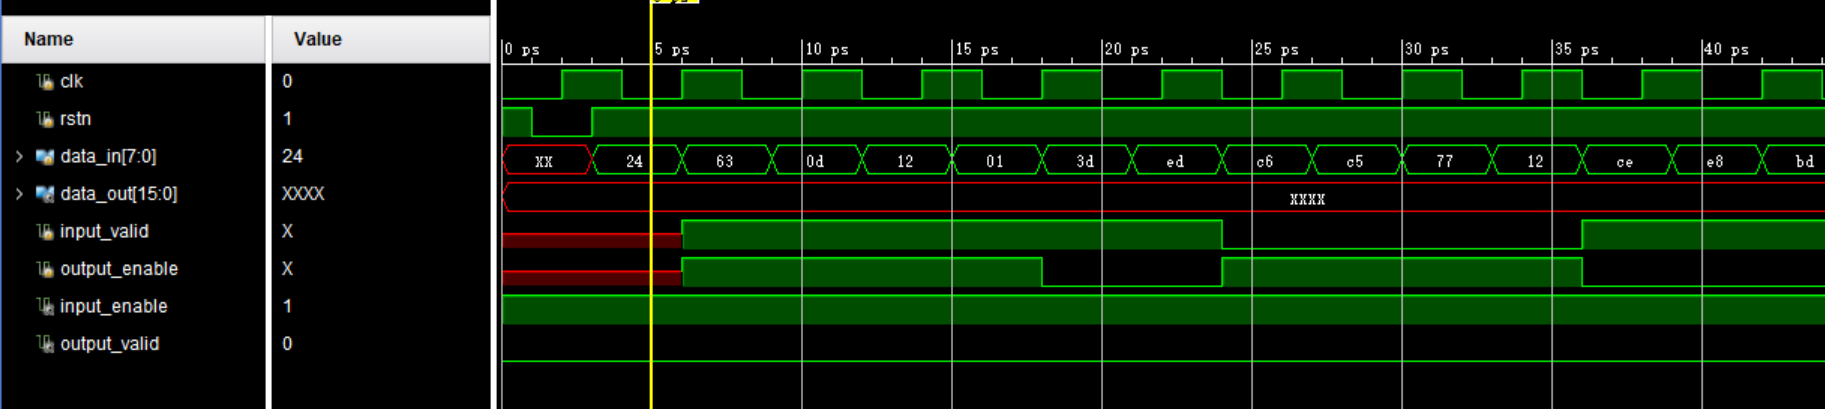
\includegraphics[width=0.98\textwidth]{assets/Fifo-0-1.png}
    \caption{先写入后读出的同步 FIFO 模块 模拟示意图: 读部分}
\end{figure}

\begin{figure}[H]
    \centering
    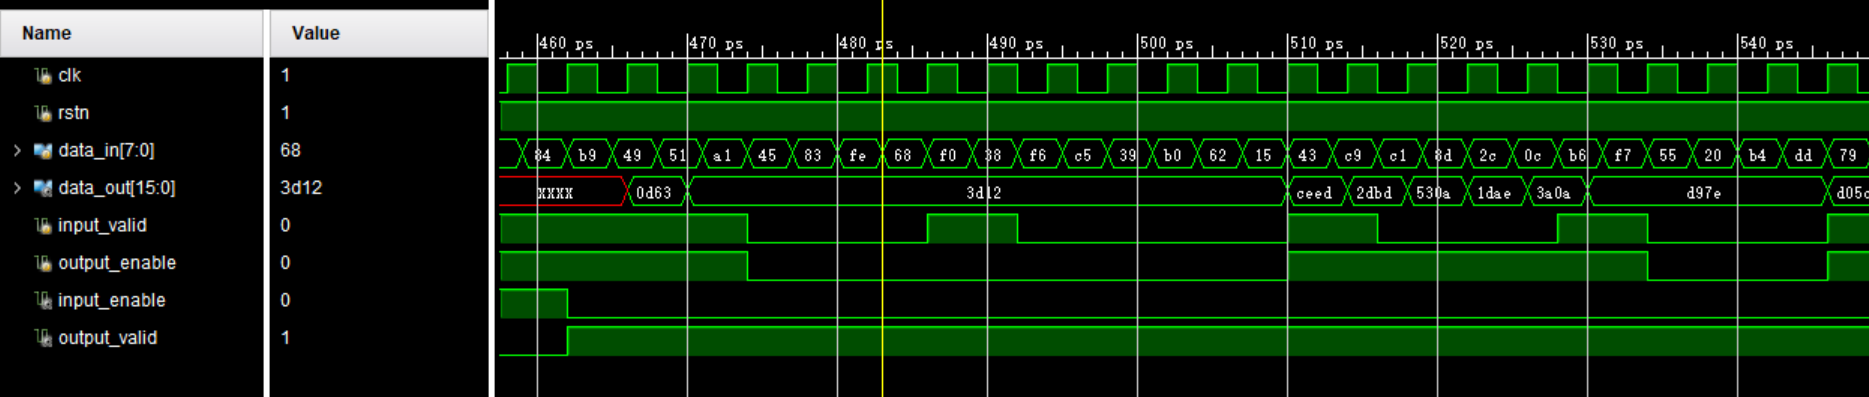
\includegraphics[width=0.98\textwidth]{assets/Fifo-0-2.png}
    \caption{先写入后读出的同步 FIFO 模块 模拟示意图: 写部分}
\end{figure}

\subsection{同步 FIFO 模块: 写入和读出同时进行}

\begin{figure}[H]
    \centering
    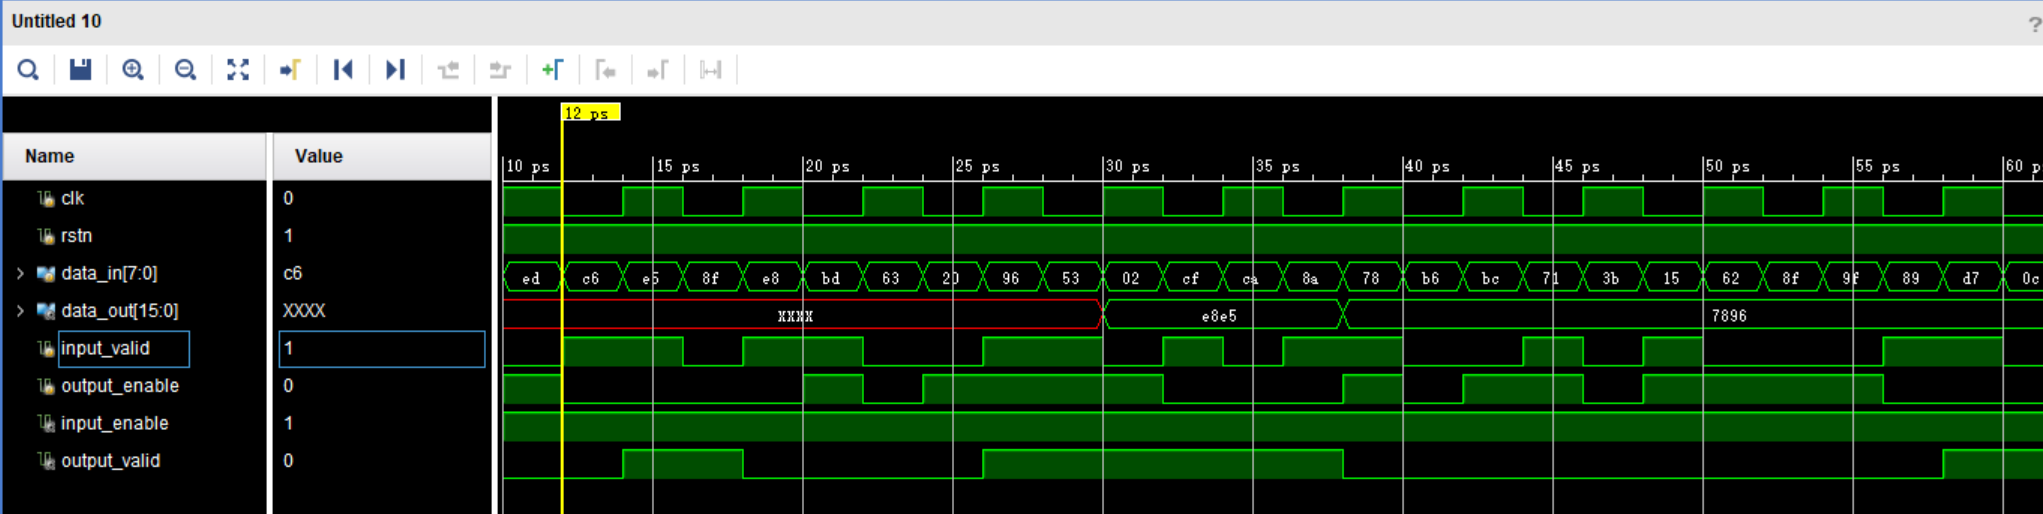
\includegraphics[width=0.98\textwidth]{assets/Fifo-1.png}
    \caption{写入和读出同时进行的同步 FIFO 模块 模拟示意图}
\end{figure}

\subsection{异步 FIFO 模块: 写入和读出同时进行}

\begin{figure}[H]
    \centering
    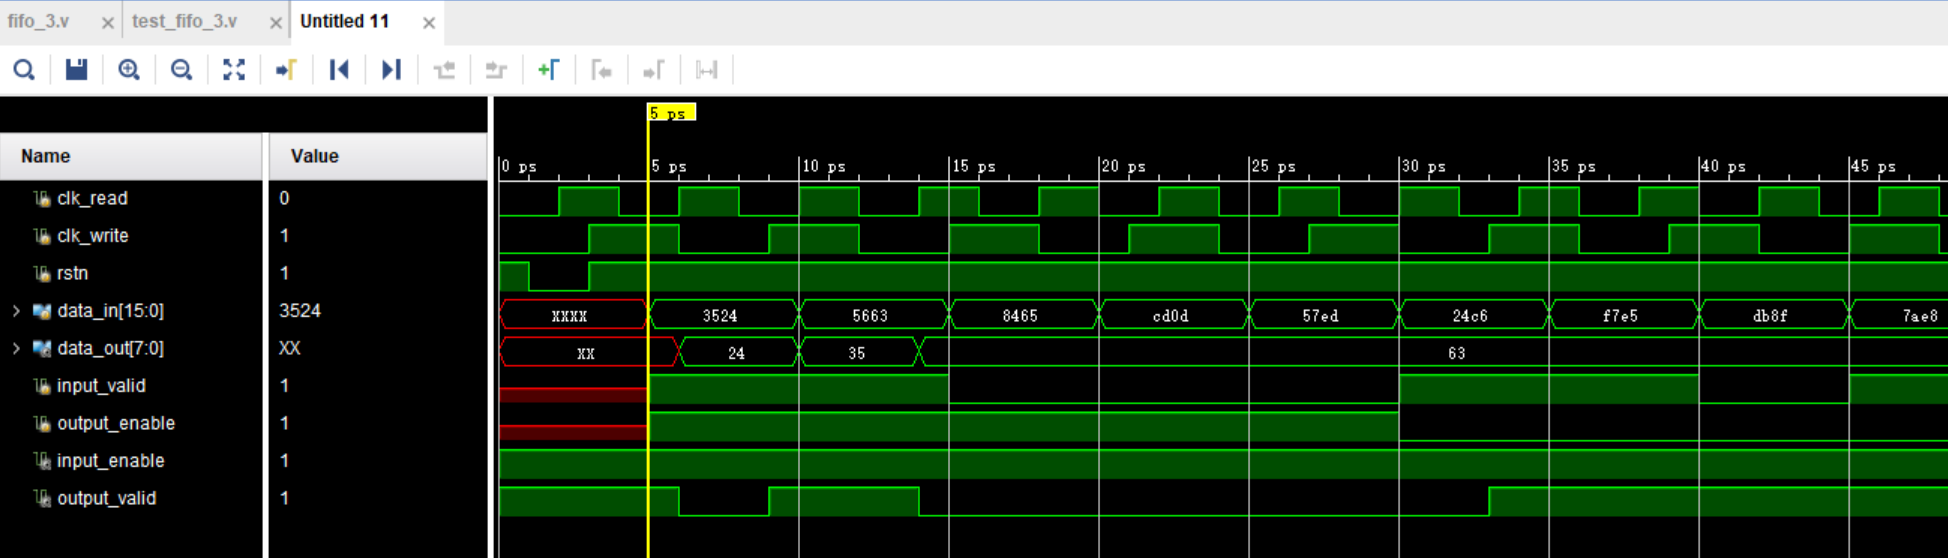
\includegraphics[width=0.98\textwidth]{assets/Fifo-2.png}
    \caption{写入和读出同时进行的异步 FIFO 模块 模拟示意图}
\end{figure}

\section{实验总结}

通过本次实验, 我了解并实践了 FIFO 的结构和设计方法, 学习了时序电路和非阻塞赋值的应用, 对时钟信号有了更深刻的了解.

\section{源代码}

\subsection{同步 FIFO 模块: 先写入后读出}

File: fifo.v
\begin{lstlisting}
    `timescale 1ps/1ps

    module fifo (
        input clk,
        input rstn,
        input [7:0] data_in,
        input input_valid,
        input output_enable,
        output reg [15:0] data_out,
        output reg input_enable,
        output reg output_valid
    );
        reg [15:0] buffer [31:0];
        // Depth=32; use buffer[i] to refer to depth i

        reg [4:0] line_write = 5'b0;
        reg [4:0] line_read = 5'b0;

        reg writeplace = 1'b0;

        always @(*) begin
            if (line_write == 5'b11111 && writeplace == 1'b1) begin
                input_enable = 0;
                output_valid = 1;
            end
            else begin
                input_enable = 1;
                output_valid = 0;
            end
        end

        always @(posedge clk or negedge rstn) begin
            if (rstn == 0) begin // 复位
                line_write <= 5'b0;
                line_read <= 5'b0;
            end
            else begin
                if (input_enable && input_valid) begin
                    if (writeplace) begin
                        buffer[line_write][15:8] <= data_in[7:0];
                        line_write <= line_write + 1;
                        writeplace <= 1'b0;
                    end
                    else begin
                        buffer[line_write][7:0] <= data_in[7:0];
                        writeplace <= 1'b1;
                    end
                end
                else if (output_enable && output_valid) begin
                    data_out[15:0] <= buffer[line_read][15:0];
                    line_read <= line_read + 1;
                end
            end
        end
    endmodule
\end{lstlisting}

File: test\_fifo.v
\begin{lstlisting}
    `timescale 1ps/1ps

    module test_fifo();
        reg clk, rstn;
        reg [7:0] data_in;
        wire [15:0] data_out;
        reg input_valid, output_enable;
        wire input_enable, output_valid;
    
        fifo inst_fifo(
            .clk(clk),
            .rstn(rstn),
            .data_in(data_in),
            .input_valid(input_valid),
            .output_enable(output_enable),
            .data_out(data_out),
            .input_enable(input_enable),
            .output_valid(output_valid)
        );
    
    
        always #2 begin
            clk = ~clk;
        end
    
        initial begin
            clk = 1'b0;
            rstn = 1'b1;
            #1 rstn = 1'b0;
            #2 rstn = 1'b1;
        end
    
        always begin
            #3;
            data_in = $random() % 9'b1_0000_0000;
        end
    
        always begin
            #6;
            input_valid = $random() % 2;
            output_enable = $random() % 2;
        end
    endmodule
\end{lstlisting}

\subsection{同步 FIFO 模块: 写入和读出同时进行}

File: fifo\_2.v
\begin{lstlisting}
    `timescale 1ps/1ps

    module fifo_2 (
        input clk,
        input rstn,
        input [7:0] data_in,
        input input_valid,
        input output_enable,
        output reg [15:0] data_out,
        output reg input_enable,
        output reg output_valid
    );
        reg [15:0] buffer [31:0];
        // Depth=32; use buffer[i] to refer to depth i
    
        reg [4:0] line_write = 5'b0;
        reg [4:0] line_read = 5'b0;
    
        reg writeplace = 1'b0;
    
        always @(*) begin
            // If there is enough to read, then read it
            if (line_write >= line_read && writeplace) begin
                output_valid = 1;
            end
            else begin
                output_valid = 0;
            end
    
            // If buffer is not full, then writing is allowed
            if (line_write == 5'b11111 && writeplace) begin
                input_enable = 0;
            end
            else begin
                input_enable = 1;
            end
        end
    
        always @(posedge clk or negedge rstn) begin
            if (rstn == 0) begin // 复位
                line_write <= 5'b0;
                line_read <= 5'b0;
            end
            else begin
                if (input_enable && input_valid) begin
                    if (writeplace) begin
                        buffer[line_write][15:8] <= data_in[7:0];
                        line_write <= line_write + 1;
                        writeplace <= 1'b0;
                    end
                    else begin
                        buffer[line_write][7:0] <= data_in[7:0];
                        writeplace <= 1'b1;
                    end
                end
    
                if (output_enable && output_valid) begin
                    if (line_write == line_read) begin
                        data_out[15:0] <= {data_in[7:0], buffer[line_read][7:0]};
                    end
                    else begin
                        data_out[15:0] <= buffer[line_read][15:0];
                        line_read <= line_read + 1;
                    end
                end
            end
        end
        
    endmodule
\end{lstlisting}

File: test\_fifo\_2.v
\begin{lstlisting}
    `timescale 1ps/1ps

    module test_fifo();
        reg clk, rstn;
        reg [7:0] data_in;
        wire [15:0] data_out;
        reg input_valid, output_enable;
        wire input_enable, output_valid;
    
        fifo_2 inst_fifo_2(
            .clk(clk),
            .rstn(rstn),
            .data_in(data_in),
            .input_valid(input_valid),
            .output_enable(output_enable),
            .data_out(data_out),
            .input_enable(input_enable),
            .output_valid(output_valid)
        );
    
    
        always #2 begin
            clk = ~clk;
        end
    
        initial begin
            clk = 1'b0;
            rstn = 1'b1;
            #1 rstn = 1'b0;
            #2 rstn = 1'b1;
        end
    
        always begin
            #3;
            data_in = $random() % 9'b1_0000_0000;
        end
    
        always begin
            #6;
            input_valid = $random() % 2;
            output_enable = $random() % 2;
        end
    endmodule
\end{lstlisting}

\subsection{异步 FIFO 模块: 写入和读出同时进行}

File: fifo\_3.v
\begin{lstlisting}
    `timescale 1ps/1ps

    module fifo_3 (
        input clk_read,
        input clk_write,
        input rstn,
        input [15:0] data_in,
        input input_valid,
        input output_enable,
        output reg [7:0] data_out,
        output reg input_enable,
        output reg output_valid
    );
        reg [15:0] buffer [31:0];
        // Depth=32; use buffer[i] to refer to depth i
    
        reg [4:0] line_write = 5'b0;
        reg [4:0] line_read = 5'b0;
    
        reg readplace = 1'b0;
    
        always @(*) begin
            // If there is enough to read, then read it
            if ((line_write > line_read) || (line_write == line_read && !readplace)) begin
                output_valid = 1;
            end
            else begin
                output_valid = 0;
            end
    
            // If buffer is not full, then writing is allowed
            if (line_write == 5'b11111) begin
                input_enable = 0;
            end
            else begin
                input_enable = 1;
            end
        end
    
        always @(posedge clk_write or negedge rstn) begin
            if (rstn == 0) begin // 复位
                line_write <= 5'b0;
            end
            else if (input_enable && input_valid) begin
                buffer[line_write][15:0] <= data_in[15:0];
                line_write <= line_write + 1;
            end
        end
    
        always @(posedge clk_read or negedge rstn) begin
            if (rstn == 0) begin // 复位
                line_read <= 5'b0;
                readplace <= 1'b0;
            end
            else if (output_enable && output_valid) begin
                if (readplace) begin
                    if (line_write == line_read && input_valid) begin
                        data_out[7:0] <= data_in[15:8];
                    end
                    else
                    begin
                        data_out[7:0] <= buffer[line_read][15:8];
                    end
                    readplace <= 1'b0;
                    line_read <= line_read + 1;
                end
                else begin
                    if (line_write == line_read && input_valid) begin
                        data_out[7:0] <= data_in[7:0];
                    end
                    else 
                    begin
                        data_out[7:0] <= buffer[line_read][7:0];
                    end
                    readplace <= 1'b1;
                end
            end
        end
    endmodule    
\end{lstlisting}

File: test\_fifo\_3.v
\begin{lstlisting}
    `timescale 1ps/1ps

    module test_fifo();
        reg clk_read, clk_write, rstn;
        reg [15:0] data_in;
        wire [7:0] data_out;
        reg input_valid, output_enable;
        wire input_enable, output_valid;
    
        fifo_3 inst_fifo_3(
            .clk_read(clk_read),
            .clk_write(clk_write),
            .rstn(rstn),
            .data_in(data_in),
            .input_valid(input_valid),
            .output_enable(output_enable),
            .data_out(data_out),
            .input_enable(input_enable),
            .output_valid(output_valid)
        );
    
    
        always #3 begin
            clk_write = ~clk_write;
        end
    
        always #2 begin
            clk_read = ~clk_read;
        end
    
        initial begin
            clk_read = 1'b0;
            clk_write = 1'b0;
            rstn = 1'b1;
            #1 rstn = 1'b0;
            #2 rstn = 1'b1;
        end
    
        always begin
            #3;
            data_in = $random() % 17'b1_0000_0000_0000_0000;
        end
    
        always begin
            #6;
            input_valid = $random() % 2;
            output_enable = $random() % 2;
        end
    endmodule
\end{lstlisting}

\end{document}